 \documentclass[border=15pt, multi, tikz]{standalone}
\usepackage{import}
\subimport{../../layers/}{init}
\usetikzlibrary{positioning}
\usetikzlibrary{3d} %for including external image 

\def\ConvColor{rgb:brown,5;yellow,2.5;black,5}
\def\ConvReluColor{rgb:orange,5;red,5;white,5}
\def\InstanceNormColor{rgb:red,1;black,5.3}

\begin{document}
\begin{tikzpicture}


\tikzstyle{connection}=[ultra thick,every node/.style={sloped,allow upside down},draw=\edgecolor,opacity=0.5]


%% Draw Layer Blocks
%%%%%%%%%%%%%%%%%%%%%%%%%%%%%%%%%%%%%%%%%%%%%%%%%%%%%%%%%%%%%%%%%%%%%%%%%%%%%%%%%%%%%%%%

\node[canvas is zy plane at x=0] (temp) at (0,0,0) {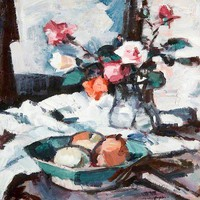
\includegraphics[width=10cm,height=10cm]{art.jpg}};

% conv1, LeakyRelu
\pic[shift={(1,0,0)}] at (0,0,0) {RightBandedBox={name=cr1,caption=Conv + ReLU,%
        xlabel={{"3","dummy"}}, ylabel=128,zlabel=128,fill=\ConvColor,bandfill=\ConvReluColor,%
        height=50,width={2},depth=50}};
        

% conv2, InstanceNorm, LeakyRelu
\pic[shift={(2.7,0,0)}] at (cr1-east) {RightBandedBox={name=cr2,caption= Conv + IN + ReLU,%
        xlabel={{"64","dummy"}},, ylabel=64,zlabel=64,,fill=\ConvColor,bandfill=\InstanceNormColor,%
        height=40,width={10},depth=40}};
        
\pic[shift={(0,0,0)}] at (cr2-east) {Box={name=r1,%
        fill=\ConvReluColor,opacity=0.8,height=40,width=1,depth=40}};


% conv3, BatchNorm, LeakyRelu
\pic[shift={(2.5,0,0)}] at (r1-east) {RightBandedBox={name=cr3,caption=Conv + IN + ReLU,%
        xlabel={{"128","dummy"}}, ylabel=32, zlabel=32,fill=\ConvColor,bandfill=\InstanceNormColor,%
        height=30,width={15},depth=30}};
        
\pic[shift={(0,0,0)}] at (cr3-east) {Box={name=r2,%
        fill=\ConvReluColor,opacity=0.8,height=30,width=1,depth=30}};
        
% conv4, BatchNorm, LeakyRelu
\pic[shift={(2,0,0)}] at (r2-east) {RightBandedBox={name=cr4,caption=Conv + IN + ReLU,%
        xlabel={{"256","dummy"}}, ylabel=16, zlabel=16,fill=\ConvColor,bandfill=\InstanceNormColor,%
        height=20,width={20},depth=20}};
        
\pic[shift={(0,0,0)}] at (cr4-east) {Box={name=r3,%
        fill=\ConvReluColor,opacity=0.8,height=20,width=1,depth=20}};
        
        
% conv5, BatchNorm, LeakyRelu
\pic[shift={(2,0,0)}] at (r3-east) {RightBandedBox={name=cr5,caption=Conv + IN + ReLU,%
        xlabel={{"512","dummy"}}, ylabel=8, zlabel=8,fill=\ConvColor,bandfill=\InstanceNormColor,%
        height=15,width={25},depth=15}};
        
\pic[shift={(0,0,0)}] at (cr5-east) {Box={name=r4,%
        fill=\ConvReluColor,opacity=0.8,height=15,width=1,depth=15}};
        
% conv6, BatchNorm, LeakyRelu
\pic[shift={(2,0,0)}] at (r4-east) {RightBandedBox={name=cr6,caption=Conv + IN + ReLU,%
        xlabel={{"1024","dummy"}}, ylabel=4, zlabel=4,fill=\ConvColor,bandfill=\InstanceNormColor,%
        height=10,width={30},depth=10}};
        
\pic[shift={(0,0,0)}] at (cr6-east) {Box={name=r5,%
        fill=\ConvReluColor,opacity=0.8,height=10,width=1,depth=10}};
        
        
% conv7
\pic[shift={(2,0,0)}] at (r5-east) {Box={name=cr7,%
        xlabel={{"1", "dummy"}},fill=\ConvColor, caption=Conv,%
        height=4,width={4},depth=4}};
 
        

%%%%%%%%%%%%%%%%%%%%%%%%%%%%%%%%%%%%%%%%%%%%%%%%%%%%%%%%%%%%%%%%%%%%%%%%%%%%%%%%%%%%%%%%
%% Draw connections
%%%%%%%%%%%%%%%%%%%%%%%%%%%%%%%%%%%%%%%%%%%%%%%%%%%%%%%%%%%%%%%%%%%%%%%%%%%%%%%%%%%%%%%%
\draw [connection]  (cr1-east)    -- node {\midarrow} (cr2-west);
\draw [connection]  (r1-east)    -- node {\midarrow} (cr3-west);
\draw [connection]  (r2-east)    -- node {\midarrow} (cr4-west);
\draw [connection]  (r3-east)    -- node {\midarrow} (cr5-west);
\draw [connection]  (r4-east)    -- node {\midarrow} (cr6-west);
\draw [connection]  (r5-east)    -- node {\midarrow} (cr7-west);

%%%%%%%%%%%%%%%%%%%%%%%%%%%%%%%%%%%%%%%%%%%%%%%%%%%%%%%%%%%%%%%%%%%%%%%%%%%%%%%%%%%%%%%%

\end{tikzpicture}
\end{document}\grid
